% Created by tikzDevice version 0.12.3.1 on 2021-08-27 12:02:10
% !TEX encoding = UTF-8 Unicode
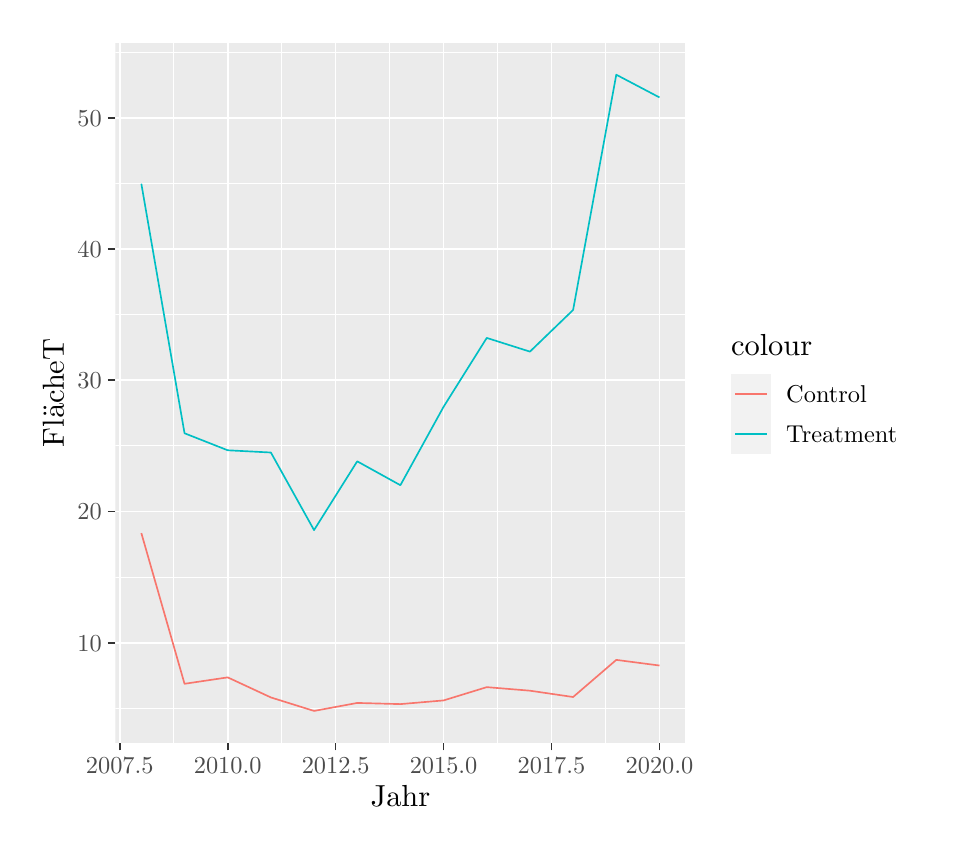
\begin{tikzpicture}[x=1pt,y=1pt]
\definecolor{fillColor}{RGB}{255,255,255}
\path[use as bounding box,fill=fillColor,fill opacity=0.00] (0,0) rectangle (325.21,289.08);
\begin{scope}
\path[clip] (  0.00,  0.00) rectangle (325.21,289.08);
\definecolor{drawColor}{RGB}{255,255,255}
\definecolor{fillColor}{RGB}{255,255,255}

\path[draw=drawColor,line width= 0.6pt,line join=round,line cap=round,fill=fillColor] (  0.00,  0.00) rectangle (325.21,289.08);
\end{scope}
\begin{scope}
\path[clip] ( 31.71, 30.69) rectangle (237.66,283.58);
\definecolor{fillColor}{gray}{0.92}

\path[fill=fillColor] ( 31.71, 30.69) rectangle (237.66,283.58);
\definecolor{drawColor}{RGB}{255,255,255}

\path[draw=drawColor,line width= 0.3pt,line join=round] ( 31.71, 43.10) --
	(237.66, 43.10);

\path[draw=drawColor,line width= 0.3pt,line join=round] ( 31.71, 90.53) --
	(237.66, 90.53);

\path[draw=drawColor,line width= 0.3pt,line join=round] ( 31.71,137.96) --
	(237.66,137.96);

\path[draw=drawColor,line width= 0.3pt,line join=round] ( 31.71,185.39) --
	(237.66,185.39);

\path[draw=drawColor,line width= 0.3pt,line join=round] ( 31.71,232.81) --
	(237.66,232.81);

\path[draw=drawColor,line width= 0.3pt,line join=round] ( 31.71,280.24) --
	(237.66,280.24);

\path[draw=drawColor,line width= 0.3pt,line join=round] ( 52.77, 30.69) --
	( 52.77,283.58);

\path[draw=drawColor,line width= 0.3pt,line join=round] ( 91.78, 30.69) --
	( 91.78,283.58);

\path[draw=drawColor,line width= 0.3pt,line join=round] (130.78, 30.69) --
	(130.78,283.58);

\path[draw=drawColor,line width= 0.3pt,line join=round] (169.79, 30.69) --
	(169.79,283.58);

\path[draw=drawColor,line width= 0.3pt,line join=round] (208.79, 30.69) --
	(208.79,283.58);

\path[draw=drawColor,line width= 0.6pt,line join=round] ( 31.71, 66.82) --
	(237.66, 66.82);

\path[draw=drawColor,line width= 0.6pt,line join=round] ( 31.71,114.24) --
	(237.66,114.24);

\path[draw=drawColor,line width= 0.6pt,line join=round] ( 31.71,161.67) --
	(237.66,161.67);

\path[draw=drawColor,line width= 0.6pt,line join=round] ( 31.71,209.10) --
	(237.66,209.10);

\path[draw=drawColor,line width= 0.6pt,line join=round] ( 31.71,256.53) --
	(237.66,256.53);

\path[draw=drawColor,line width= 0.6pt,line join=round] ( 33.27, 30.69) --
	( 33.27,283.58);

\path[draw=drawColor,line width= 0.6pt,line join=round] ( 72.28, 30.69) --
	( 72.28,283.58);

\path[draw=drawColor,line width= 0.6pt,line join=round] (111.28, 30.69) --
	(111.28,283.58);

\path[draw=drawColor,line width= 0.6pt,line join=round] (150.29, 30.69) --
	(150.29,283.58);

\path[draw=drawColor,line width= 0.6pt,line join=round] (189.29, 30.69) --
	(189.29,283.58);

\path[draw=drawColor,line width= 0.6pt,line join=round] (228.30, 30.69) --
	(228.30,283.58);
\definecolor{drawColor}{RGB}{0,191,196}

\path[draw=drawColor,line width= 0.6pt,line join=round] ( 41.07,232.69) --
	( 56.68,142.52) --
	( 72.28,136.37) --
	( 87.88,135.56) --
	(103.48,107.53) --
	(119.08,132.38) --
	(134.68,123.75) --
	(150.29,152.09) --
	(165.89,176.97) --
	(181.49,172.02) --
	(197.09,187.07) --
	(212.69,272.08) --
	(228.30,263.87);
\definecolor{drawColor}{RGB}{248,118,109}

\path[draw=drawColor,line width= 0.6pt,line join=round] ( 41.07,106.46) --
	( 56.68, 51.99) --
	( 72.28, 54.31) --
	( 87.88, 47.06) --
	(103.48, 42.18) --
	(119.08, 45.07) --
	(134.68, 44.65) --
	(150.29, 45.98) --
	(165.89, 50.78) --
	(181.49, 49.50) --
	(197.09, 47.21) --
	(212.69, 60.63) --
	(228.30, 58.59);
\end{scope}
\begin{scope}
\path[clip] (  0.00,  0.00) rectangle (325.21,289.08);
\definecolor{drawColor}{gray}{0.30}

\node[text=drawColor,anchor=base east,inner sep=0pt, outer sep=0pt, scale=  0.88] at ( 26.76, 63.79) {10};

\node[text=drawColor,anchor=base east,inner sep=0pt, outer sep=0pt, scale=  0.88] at ( 26.76,111.21) {20};

\node[text=drawColor,anchor=base east,inner sep=0pt, outer sep=0pt, scale=  0.88] at ( 26.76,158.64) {30};

\node[text=drawColor,anchor=base east,inner sep=0pt, outer sep=0pt, scale=  0.88] at ( 26.76,206.07) {40};

\node[text=drawColor,anchor=base east,inner sep=0pt, outer sep=0pt, scale=  0.88] at ( 26.76,253.50) {50};
\end{scope}
\begin{scope}
\path[clip] (  0.00,  0.00) rectangle (325.21,289.08);
\definecolor{drawColor}{gray}{0.20}

\path[draw=drawColor,line width= 0.6pt,line join=round] ( 28.96, 66.82) --
	( 31.71, 66.82);

\path[draw=drawColor,line width= 0.6pt,line join=round] ( 28.96,114.24) --
	( 31.71,114.24);

\path[draw=drawColor,line width= 0.6pt,line join=round] ( 28.96,161.67) --
	( 31.71,161.67);

\path[draw=drawColor,line width= 0.6pt,line join=round] ( 28.96,209.10) --
	( 31.71,209.10);

\path[draw=drawColor,line width= 0.6pt,line join=round] ( 28.96,256.53) --
	( 31.71,256.53);
\end{scope}
\begin{scope}
\path[clip] (  0.00,  0.00) rectangle (325.21,289.08);
\definecolor{drawColor}{gray}{0.20}

\path[draw=drawColor,line width= 0.6pt,line join=round] ( 33.27, 27.94) --
	( 33.27, 30.69);

\path[draw=drawColor,line width= 0.6pt,line join=round] ( 72.28, 27.94) --
	( 72.28, 30.69);

\path[draw=drawColor,line width= 0.6pt,line join=round] (111.28, 27.94) --
	(111.28, 30.69);

\path[draw=drawColor,line width= 0.6pt,line join=round] (150.29, 27.94) --
	(150.29, 30.69);

\path[draw=drawColor,line width= 0.6pt,line join=round] (189.29, 27.94) --
	(189.29, 30.69);

\path[draw=drawColor,line width= 0.6pt,line join=round] (228.30, 27.94) --
	(228.30, 30.69);
\end{scope}
\begin{scope}
\path[clip] (  0.00,  0.00) rectangle (325.21,289.08);
\definecolor{drawColor}{gray}{0.30}

\node[text=drawColor,anchor=base,inner sep=0pt, outer sep=0pt, scale=  0.88] at ( 33.27, 19.68) {2007.5};

\node[text=drawColor,anchor=base,inner sep=0pt, outer sep=0pt, scale=  0.88] at ( 72.28, 19.68) {2010.0};

\node[text=drawColor,anchor=base,inner sep=0pt, outer sep=0pt, scale=  0.88] at (111.28, 19.68) {2012.5};

\node[text=drawColor,anchor=base,inner sep=0pt, outer sep=0pt, scale=  0.88] at (150.29, 19.68) {2015.0};

\node[text=drawColor,anchor=base,inner sep=0pt, outer sep=0pt, scale=  0.88] at (189.29, 19.68) {2017.5};

\node[text=drawColor,anchor=base,inner sep=0pt, outer sep=0pt, scale=  0.88] at (228.30, 19.68) {2020.0};
\end{scope}
\begin{scope}
\path[clip] (  0.00,  0.00) rectangle (325.21,289.08);
\definecolor{drawColor}{RGB}{0,0,0}

\node[text=drawColor,anchor=base,inner sep=0pt, outer sep=0pt, scale=  1.10] at (134.68,  7.64) {Jahr};
\end{scope}
\begin{scope}
\path[clip] (  0.00,  0.00) rectangle (325.21,289.08);
\definecolor{drawColor}{RGB}{0,0,0}

\node[text=drawColor,rotate= 90.00,anchor=base,inner sep=0pt, outer sep=0pt, scale=  1.10] at ( 13.08,157.13) {FlächeT};
\end{scope}
\begin{scope}
\path[clip] (  0.00,  0.00) rectangle (325.21,289.08);
\definecolor{fillColor}{RGB}{255,255,255}

\path[fill=fillColor] (248.66,129.57) rectangle (319.71,184.69);
\end{scope}
\begin{scope}
\path[clip] (  0.00,  0.00) rectangle (325.21,289.08);
\definecolor{drawColor}{RGB}{0,0,0}

\node[text=drawColor,anchor=base west,inner sep=0pt, outer sep=0pt, scale=  1.10] at (254.16,170.55) {colour};
\end{scope}
\begin{scope}
\path[clip] (  0.00,  0.00) rectangle (325.21,289.08);
\definecolor{fillColor}{gray}{0.95}

\path[fill=fillColor] (254.16,149.53) rectangle (268.61,163.98);
\end{scope}
\begin{scope}
\path[clip] (  0.00,  0.00) rectangle (325.21,289.08);
\definecolor{drawColor}{RGB}{248,118,109}

\path[draw=drawColor,line width= 0.6pt,line join=round] (255.60,156.75) -- (267.17,156.75);
\end{scope}
\begin{scope}
\path[clip] (  0.00,  0.00) rectangle (325.21,289.08);
\definecolor{drawColor}{RGB}{248,118,109}

\path[draw=drawColor,line width= 0.6pt,line join=round] (255.60,156.75) -- (267.17,156.75);
\end{scope}
\begin{scope}
\path[clip] (  0.00,  0.00) rectangle (325.21,289.08);
\definecolor{fillColor}{gray}{0.95}

\path[fill=fillColor] (254.16,135.07) rectangle (268.61,149.53);
\end{scope}
\begin{scope}
\path[clip] (  0.00,  0.00) rectangle (325.21,289.08);
\definecolor{drawColor}{RGB}{0,191,196}

\path[draw=drawColor,line width= 0.6pt,line join=round] (255.60,142.30) -- (267.17,142.30);
\end{scope}
\begin{scope}
\path[clip] (  0.00,  0.00) rectangle (325.21,289.08);
\definecolor{drawColor}{RGB}{0,191,196}

\path[draw=drawColor,line width= 0.6pt,line join=round] (255.60,142.30) -- (267.17,142.30);
\end{scope}
\begin{scope}
\path[clip] (  0.00,  0.00) rectangle (325.21,289.08);
\definecolor{drawColor}{RGB}{0,0,0}

\node[text=drawColor,anchor=base west,inner sep=0pt, outer sep=0pt, scale=  0.88] at (274.11,153.72) {Control};
\end{scope}
\begin{scope}
\path[clip] (  0.00,  0.00) rectangle (325.21,289.08);
\definecolor{drawColor}{RGB}{0,0,0}

\node[text=drawColor,anchor=base west,inner sep=0pt, outer sep=0pt, scale=  0.88] at (274.11,139.27) {Treatment};
\end{scope}
\end{tikzpicture}
